\documentclass[11pt]{article}
    \title{\textbf{Práctica 3}}
    \author{Adrián Racero Serrano}
    \date{}
    
    \addtolength{\topmargin}{-3cm}
    \addtolength{\textheight}{3cm}
\usepackage{graphicx}
\usepackage{whilecode2}
\usepackage{algorithmic}
\begin{document}

\maketitle
\thispagestyle{empty}

\section*{Ejercicio 1}
\begin{figure}[htp]
\centering
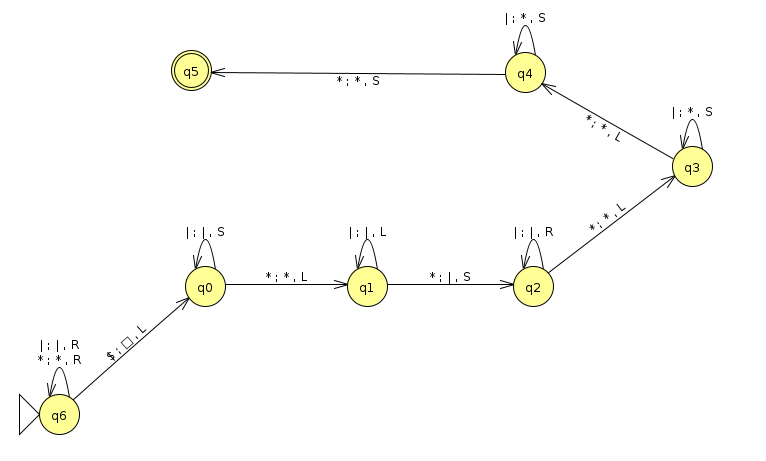
\includegraphics[scale=0.60]{ejercicio1.png}
\end{figure} 

\newpage

\section*{Ejercicio 2}
\begin{center}$<<\pi^1_1|\sigma\left(\pi^3_3\right)>|\sigma\left(\pi^4_4\right)>$
\\\end{center}
\begin{figure}[htp]
\centering
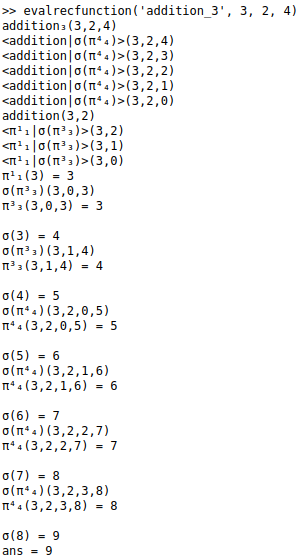
\includegraphics[scale=0.70]{ejemplo_ejecucion.png}
\label{}
\end{figure}

\newpage

\section*{Ejercicio 3}
\begin{whilecode}[H]
$addition3=(3, s)$
\\
$s:$
\\
 \While{$X_3 \not = 0$}{

  $X_2 \Assig X_2 + 1$\;
  $X_3 \Assig X_3 - 1$\;

 }
 \While{$X_2 \not = 0$}{

  $X_1 \Assig X_1 + 1$\;
  $X_2 \Assig X_2 - 1$\;

 }
\end{whilecode}

\end{document}

